\documentclass{beamer}

\mode<presentation> {

%\usetheme{default}
%\usetheme{AnnArbor}
%\usetheme{Antibes}
%\usetheme{Bergen}
%\usetheme{Berkeley}
%\usetheme{Berlin}
%\usetheme{Boadilla}
%\usetheme{CambridgeUS}
%\usetheme{Copenhagen}
%\usetheme{Darmstadt}
%\usetheme{Dresden}
%\usetheme{Frankfurt}
%\usetheme{Goettingen}
%\usetheme{Hannover}
%\usetheme{Ilmenau}
%\usetheme{JuanLesPins}
%\usetheme{Luebeck}
\usetheme{Madrid}
%\usetheme{Malmoe}
%\usetheme{Marburg}
%\usetheme{Montpellier}
%\usetheme{PaloAlto}
%\usetheme{Pittsburgh}
%\usetheme{Rochester}
%\usetheme{Singapore}
%\usetheme{Szeged}
%\usetheme{Warsaw}


%\usecolortheme{albatross}
%\usecolortheme{beaver}
%\usecolortheme{beetle}
%\usecolortheme{crane}
%\usecolortheme{dolphin}
%\usecolortheme{dove}
%\usecolortheme{fly}
%\usecolortheme{lily}
%\usecolortheme{orchid}
%\usecolortheme{rose}
%\usecolortheme{seagull}
%\usecolortheme{seahorse}
%\usecolortheme{whale}
%\usecolortheme{wolverine}

%\setbeamertemplate{footline} % To remove the footer line in all slides uncomment this line
%\setbeamertemplate{footline}[page number] % To replace the footer line in all slides with a simple slide count uncomment this line

%\setbeamertemplate{navigation symbols}{} % To remove the navigation symbols from the bottom of all slides uncomment this line
}

\usepackage{graphicx} % Allows including images
\usepackage{booktabs} % Allows the use of \toprule, \midrule and \bottomrule in tables
\usepackage{amsfonts}
\usepackage{mathrsfs, bbold}
\usepackage{amsmath,amssymb,graphicx}
\usepackage{mathtools} % gather
\usepackage[export]{adjustbox} % right-aligned graphics

% argmax
\DeclareMathOperator*{\argmax}{arg\,max}

%----------------------------------------------------------------------------------------
%	TITLE PAGE
%----------------------------------------------------------------------------------------

\title["23"]{23: Dirichlet Process Models}

\author{Taylor} 
\institute[UVA] 
{
University of Virginia \\
\medskip
\textit{} 
}
\date{} 

\begin{document}
%----------------------------------------------------------------------------------------

\begin{frame}
\titlepage 
\end{frame}

%----------------------------------------------------------------------------------------
\begin{frame}
\frametitle{Introduction}

We'll take a look at {\bf Dirichlet Processes} now, and see how they're useful for mixture modeling.

\end{frame}
%----------------------------------------------------------------------------------------
\begin{frame}
\frametitle{Bayesian histograms}

A probability model for the density analagous to the histogram 
$$
f(y \mid \pi_1, \ldots, \pi_k) = \sum_{h=1}^k 1_{\xi_{h-1} < y \le \xi_{h} } \frac{\pi_h}{(\xi_{h} - \xi_{h-1})}
$$
where $\xi_0 < \xi_1 < \cdots < \xi_k$ are your {\bf knot points}, and $(\pi_1, \ldots, \pi_k)$ is an unknown probability vector. 
\newline
\pause

Note
$$
\int f(y) \text{d}y = \sum_{h=1}^k \text{base}_h \times \text{height}_h = \sum_{h=1}^k (\xi_{h} - \xi_{h-1})\frac{\pi_h}{(\xi_{h} - \xi_{h-1})} = 1.
$$

\end{frame}


%----------------------------------------------------------------------------------------
\begin{frame}
\frametitle{Bayesian histograms}

$$
f(y \mid \pi) = \sum_{h=1}^k 1_{\xi_{h-1} < y \le \xi_{h} } \frac{\pi_h}{(\xi_{h} - \xi_{h-1})}
$$
We can put a $\text{Dirichlet}(\alpha_1, \ldots, \alpha_k)$ prior on the parameters $\pi = (\pi_1, \ldots, \pi_k)$:

$$
p(\pi ) = \frac{\Gamma\left( \sum_{h=1}^k a_h \right) }{\prod_{h=1}^k \Gamma(\alpha_h) } \prod_{h=1}^k \pi_h^{a_h-1}
$$
where $a = (a_1, \ldots, a_k)$ are the chosen parameters of the prior.

\end{frame}

%----------------------------------------------------------------------------------------
\begin{frame}
\frametitle{Bayesian histograms}

Note that $f(y \mid \pi)$ was for one data point $y$. Let $\sigma(i) = \{k : \xi_{k-1} < y_i \le \xi_{k} \}$. Notice that this function is many-to-one. Then

\begin{align*}
p(y \mid \pi)  &= \prod_{i=1}^n f(y_i \mid \pi) \\
&= \prod_{i=1}^n\left[ \sum_{h=1}^k 1_{\xi_{h-1} < y_i \le \xi_{h} } \frac{\pi_h}{(\xi_{h} - \xi_{h-1})} \right] \\
&= \prod_{i=1}^n\left[  \frac{\pi_{\sigma(i)} }{(\xi_{\sigma(i)} - \xi_{\sigma(i)-1}  )} \right] \\
&= \prod_{h=1}^k \left[  \frac{\pi_{h} }{(\xi_{h} - \xi_{h-1}  )} \right] ^{n_h}
\end{align*}  
where $n_h = \sum_{i=1}^n 1_{\xi_{h-1} < y_i \le \xi_{h} }$.
\end{frame}

%----------------------------------------------------------------------------------------
\begin{frame}
\frametitle{Bayesian histograms}

Bayes' rule:

\begin{align*}
p(\pi \mid y) &\propto p(y \mid \pi) p(\pi) \\
&= \left[\prod_{h=1}^k   \left(\frac{\pi_{h} }{(\xi_{h} - \xi_{h-1}  )}\right)  ^{n_h} \right]\prod_{h=1}^k \pi_h^{a_h-1} \\
&\propto \prod_{h=1}^k \pi_h^{a_h+n_h-1}
\end{align*}
So $p(\pi \mid y) = \text{Dirichlet}(a_1 + n_1, \ldots, a_k + n_k)$.
\pause
\newline

But bin specification is annoying!
\end{frame}

%----------------------------------------------------------------------------------------
\begin{frame}
\frametitle{A quick note}

If $\pi \sim \text{Dirichlet}(a_1, \ldots, a_k)$ then
$$
E[\pi] = \left(\frac{a_1}{\alpha}, \cdots, \frac{a_k}{\alpha} \right)
$$
where 
$$
\alpha = a_1 + \cdots + a_k.
$$
So we can write 
$$
\pi \sim \text{Dirichlet}(\alpha E[\pi])
$$
as well. $\alpha$ has the interpretation of a sample size.

\end{frame}

%----------------------------------------------------------------------------------------
\begin{frame}
\frametitle{Definitions}

A {\bf random probability measure} assigns probabilities to sets, and they still satisfy the three probability axioms, but these probabilities are random. 
\newline
\pause

The random probability measure $P$ is a {\bf Dirichlet process} if for {\bf any} measurable partition $B_1, \ldots, B_k$ of a sample space $\Omega$, the vector
$$
P(B_1), \ldots, P(B_k) \sim \text{Dirichlet}(\alpha P_0(B_1), \ldots, \alpha P_0(B_k)).
$$


\end{frame}
%----------------------------------------------------------------------------------------
\begin{frame}
\frametitle{Definitions}


\begin{enumerate}
\item $P_0$ is a {\bf baseline probability measure} we pick (e.g. normal)
\item shorthand: $P \sim \text{DP}(\alpha P_0)$
\item $P(B) \sim \text{Beta}(\alpha P_0(B), \alpha(1-P_0(B)))$ for any measurable $B$
\item $E[P(B)] = P_0(B)$
\item $V[P(B)] = P_0(B)[1-P_0(B)]/(1+\alpha)$
\end{enumerate}

\end{frame}

%----------------------------------------------------------------------------------------
\begin{frame}
\frametitle{Returning to the Bayesian histogram}

Assume $y_i \overset{iid}{\sim} P$ and $P \sim \text{DP}(\alpha P_0)$. Then, for any partition $B_1, \ldots, B_k$,  
\begin{align*}
&P(B_1), \ldots, P(B_k) \mid y_1, \ldots, y_n \\
&\sim \text{Dirichlet}\left(\alpha P_0(B_1) + \sum_{i=1}^n 1_{y_i \in B_1}, \ldots, \alpha P_0(B_k) + \sum_{i=1}^n 1_{y_i \in B_k} \right)
\end{align*}
using the same reasoning as in slide 5 (let $B_i = \xi_i - \xi_{i-1}$).
\newline
\pause

What happens when we take the noninformative prior $\alpha \downarrow 0$?

\end{frame}


%----------------------------------------------------------------------------------------
\begin{frame}
\frametitle{Returning to the Bayesian histogram}

In particular, for any measurable $B$, $P(B)\mid y_1, \ldots, y_n$ follows a 
$$
\text{Beta}\left(\alpha P_0(B) + \sum_{i=1}^n 1_{y_i \in B},  \alpha + n -  \left[ \alpha P_0(B) + \sum_{i=1}^n 1_{y_i \in B} \right] \right)
$$
and
\begin{align*}
E[P(B) \mid y_1, \ldots, y_n ] 
&= \frac{\alpha P_0(B) + \sum_{i=1}^n 1_{y_i \in B}}{\alpha + n} \\
&= \frac{\alpha }{\alpha + n}P_0(B)  + \frac{n}{\alpha + n}\sum_{i=1}^n \frac{1_{y_i \in B}}{n}
\end{align*}
\pause

not ``smooth" even if $P_0$ was!

\end{frame}

%----------------------------------------------------------------------------------------
\begin{frame}
\frametitle{The stick-breaking representation}

We can write a DP as a countably infinite mixture of point masses:
$$
P(\cdot) = \sum_{h=1}^{\infty} \pi_h \delta_{\theta_h}(\cdot).
$$

Round 1
\begin{enumerate}
\item sample location $\theta_1 \sim P_0$
\item sample associated probability $V_1 \sim \text{Uniform}(0,1)$
\item we have $1-V_1$ probability left over...
\end{enumerate}
\pause

Round 2
\begin{enumerate}
\item sample location $\theta_2 \sim P_0$
\item sample $V_2 \sim \text{Uniform}(0,1)$
\item probability at second location is now $(1-V_1)V_2$
\item we have $1-(V_1 + V_2(1-V_1)) = 1-V_1 - V_2(1-V_1) = (1-V_1)(1-V_2)$ probability left over...
\end{enumerate}

\end{frame}


%----------------------------------------------------------------------------------------
\begin{frame}
\frametitle{The stick-breaking representation}

We can write a DP as a countably infinite mixture of point masses:
$$
P(\cdot) = \sum_{h=1}^{\infty} \pi_h \delta_{\theta_h}(\cdot).
$$
with
$$
\pi_h = V_h \prod_{l < h}(1-V_l)
$$
and $V_h \overset{\text{iid}}{\sim} \text{Beta}(1,\alpha)$, $\theta_h \overset{\text{iid}}{\sim} P_0$

\end{frame}
%----------------------------------------------------------------------------------------
\begin{frame}
\frametitle{The stick-breaking representation}

\begin{center}
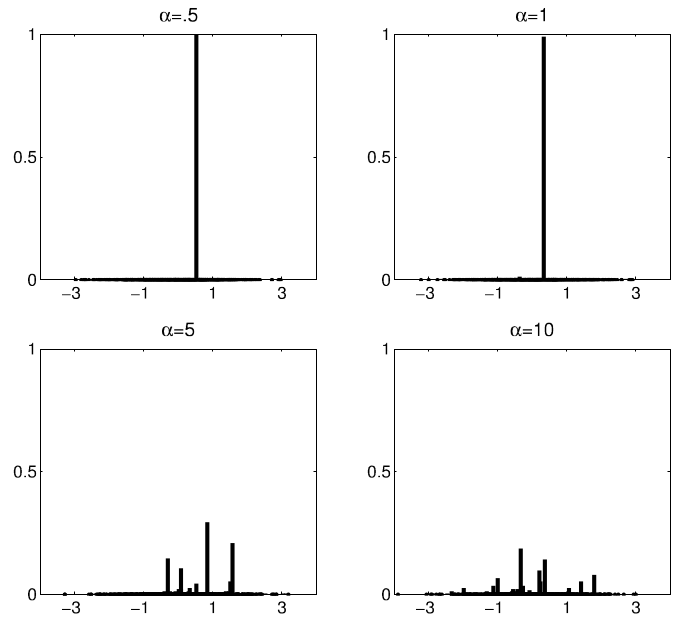
\includegraphics[width=80mm]{stick_breaking.png}
\end{center}


\end{frame}


%----------------------------------------------------------------------------------------
\begin{frame}
\frametitle{The stick-breaking representation}


\begin{align*}
E[P(B)] &= \sum_{h=1}^{\infty} E[\pi_h 1_{\theta_h \in B}]\\
&= \sum_{h=1}^{\infty} E[\pi_h] E[1_{\theta_h \in B}] \\
&= \sum_{h=1}^{\infty} E[V_h \prod_{l < h}(1-V_l)] P_0(B) \\
&= P_0(B) \sum_{h=1}^{\infty} E[V_h] \prod_{l < h}E[(1-V_l)] \\
&= P_0(B) \sum_{h=1}^{\infty} \frac{1}{1+\alpha}\left(\frac{\alpha}{1+\alpha}  \right)^{h-1}\\
&= P_0(B) 
\end{align*}

\end{frame}

%----------------------------------------------------------------------------------------
\begin{frame}
\frametitle{Dirichlet process mixtures}

Sampling $P \sim \text{DP}(\alpha P_0)$ and then using that random histogram as the distribution for a sample of continuous $y_i$ random variables is problematic because we would like $P$ to be smooth. 
\newline
\pause

We can use DPs for {\bf general kernel mixture models} though:
\begin{align*}
f(y \mid P) &= \int \mathcal{K}(y \mid \theta) P( \text{d} \theta) \\
&= \sum_{h=1}^{\infty} \pi_h \mathcal{K}(y \mid \theta_h)
\end{align*}

This is a mixture model, but there are an infinite number of mixands!

\end{frame}


\end{document} 
